\documentclass{article}
\usepackage{amsmath}
\usepackage{tikz}

\title{Golden Article Test}
\author{Texly Testing Suite}
\date{\today}

\begin{document}
\maketitle

\section{Introduction}
Testing standard PDF generation with mathematics and figures.
\begin{equation}
e^{i\pi} + 1 = 0
\end{equation}

\section{TikZ Diagram}
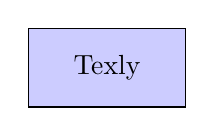
\begin{tikzpicture}
  \draw[fill=blue!20] (0,0) rectangle (2,1);
  \node at (1,0.5) {Texly};
\end{tikzpicture}

\section{Citations}
Referencing foundational work \cite{knuth1984}.

\bibliographystyle{plain}
\bibliography{references}

\end{document}

